\documentclass[12pt]{article}
\usepackage[utf8]{inputenc}
\usepackage{geometry}
\geometry{a4paper, margin=1in}
\usepackage{enumitem}
\usepackage{titlesec}
\usepackage{graphicx}
\titleformat{\section}{\normalfont\Large\bfseries}{\thesection}{1em}{}
\titleformat{\subsection}{\normalfont\large\bfseries}{\thesubsection}{1em}{}

\begin{document}

\begin{titlepage}
   \begin{center}
       \vspace*{1cm}

       \textbf{Software Design Document (SDD)}
        \author{Group 4}
        \date{12/10/2024}
        
        \textbf{Project Title:} Smart Dashboard \\
        \textbf{Version:} 4.0 \\
        \textbf{Date:} 12/10/2024 \\
        \textbf{Prepared By:} Group 4 \\
        \textbf{Approved By:} J. Valenzuela \\
        \textbf{Confidentiality Notice:} This document contains confidential information intended for authorized personnel only.
            
       \vspace{1.5cm}

       \textbf{Leonardo Granados-Castillo\\Armine Rad\\Benjamin Saucedo\\Ryan Takeshita}

       \vfill
            
            
       \vspace{0.8cm}

       California State University, Los Angeles\\
       11 December 2024
            
   \end{center}
\end{titlepage}

\newpage

\tableofcontents

\newpage

\section{Versions Table}
\begin{tabular}{|l|l|p{5cm}|l|l|}
\hline
\textbf{Version} & \textbf{Date} & \textbf{Changes} & \textbf{Modified By} & \textbf{Approved By} \\ \hline
1.0 & 09/07/2024 & Initial Draft & Group 4 & J. Valenzuela \\ \hline
2.0 & 10/08/2024 & Added architecture diagrams, initial UI designs & Group 4 & J. Valenzuela \\ \hline
3.0 & 11/09/2024 & Enhanced database design, expanded glossary & Group 4 & J. Valenzuela \\ \hline
4.0 & 12/10/2024 & Finalized security concerns and high-level architecture & Group 4 & J. Valenzuela \\ \hline
\end{tabular}

\newpage

\section{Introduction}
\subsection{Purpose}
The \textbf{Smart Dashboard} consolidates user and system errors from various sources into a centralized interface. Its primary objectives are:
\begin{itemize}
    \item \textbf{Efficiency:} Provide an intuitive tool for service desk staff to address errors promptly.
    \item \textbf{Scalability:} Accommodate multiple tenants with different lines of business.
    \item \textbf{Security:} Ensure sensitive data is displayed appropriately based on user access levels.
\end{itemize}

\subsection{Intended Audience}
\begin{itemize}
    \item \textbf{Developers:} Implement and maintain the system.
    \item \textbf{Admins and Service Desk Staff:} Use the dashboard for error investigation.
    \item \textbf{Stakeholders:} Understand the system’s value and functionality.
\end{itemize}

\subsection{Overview}
The \textbf{Smart Dashboard} integrates with APIs and databases (SQL Server and Oracle) to display error data in an organized, secure, and accessible manner. It adheres to QTC’s branding and UI/UX standards.

\newpage

\section{System Architecture}
\subsection{Workflow}
The architecture follows an MVC pattern:
\begin{enumerate}
    \item \textbf{Error Consolidation:} Data from APIs and databases is gathered.
    \item \textbf{Processing:} Data is categorized into user and system errors.
    \item \textbf{UI Rendering:} Data is displayed with options for sorting, filtering, and pagination.
\end{enumerate}

\textbf{Workflow Diagram:}  
\begin{figure}[h]
    \centering
    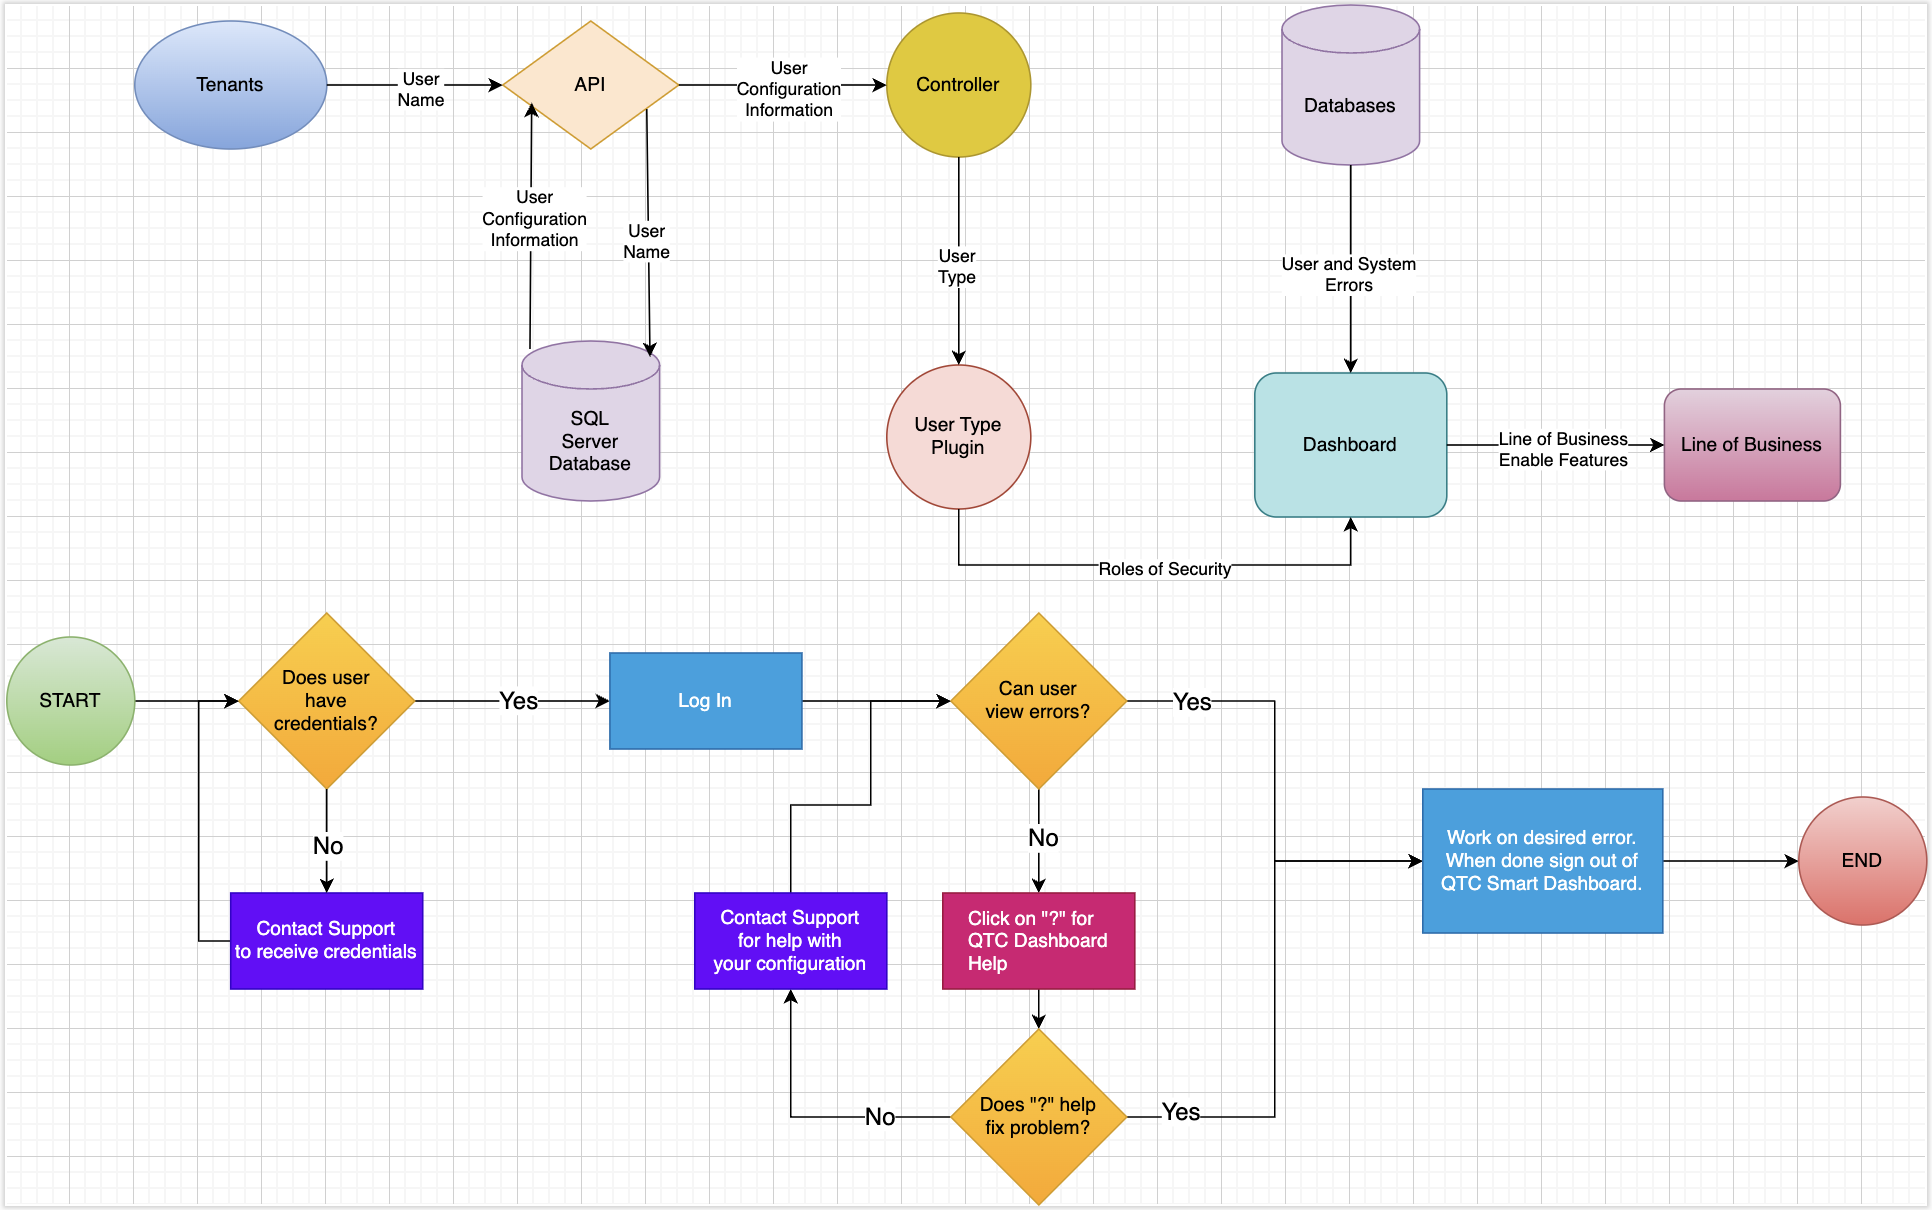
\includegraphics[width=0.8\textwidth]{workflowdiagram.png}
    \caption{Workflow Diagram} 
    \label{fig:workflow_diagram}
\end{figure}

\subsection{Site Breakdown}
\begin{itemize}
    \item \textbf{Dashboard Module:} Displays error data.
    \item \textbf{Authentication Module:} Manages user access based on roles.
    \item \textbf{Database Module:} Retrieves data for display.
\end{itemize}

\subsection{Data Storage}
The dashboard uses SQL Server for structured data storage. Key tables include:
\begin{itemize}
    \item \textbf{Error Logs:} Captures all errors.
    \item \textbf{User Roles:} Defines permissions.
    \item \textbf{Audit Trails:} Tracks user activity.
\end{itemize}

\subsection{Security Concerns}
\begin{itemize}
    \item \textbf{Role-Based Access Control:} Ensures sensitive data is visible only to authorized users.
    \item \textbf{Data Encryption:} Protects data in transit and at rest.
    \item \textbf{Error Logs:} Prevents modification of original error data.
\end{itemize}

\newpage

\section{User Interface}
\subsection{How to Use}
\begin{itemize}
    \item \textbf{Navigation:} Use the side menu to access error categories.
    \item \textbf{Search:} Filter errors using keywords or error types.
    \item \textbf{Help Section:} Provides guidance on dashboard usage.
\end{itemize}

\subsection{Database Explanation}
\begin{itemize}
    \item \textbf{Structure:} Errors are categorized by severity, type, and source.
    \item \textbf{Access Control:} Determines the visibility of specific error types.
\end{itemize}

\subsection{Interface Features}
\begin{itemize}
    \item \textbf{Pagination:} Allows users to view error entries in batches of up to 200 records per page.
    \item \textbf{Side Navigation:} Provides collapsible navigation for key dashboard sections (e.g., Dashboard, User Errors).
    \item \textbf{Help Button:} Offers contextual help, FAQs, and support options.
    \item \textbf{Advanced Filtering:} Enables users to filter data by criteria like date ranges, error types, and roles.
\end{itemize}

\newpage

\section{Glossary}
\begin{tabular}{|l|p{10cm}|}
\hline
\textbf{Term} & \textbf{Definition} \\ \hline
API & Application Programming Interface \\ \hline
DB & Database \\ \hline
MVC & Model-View-Controller \\ \hline
QTC & Quality Technical Corporation \\ \hline
SDD & Software Design Document \\ \hline
\end{tabular}

\section{References}
\begin{itemize}
    \item Dashboard SDD, QTC Team
    \item Software Requirements Specification, QTC Team
    \item Ascent Resources: Diagrams, ER Models, Workflow Overview
\end{itemize}

\end{document}